% Numbers in Sections VII-VIII come from results/v3_fix1/*.csv of the Satellite_Optical_GitHub_Publish project
% (tools/analyze_v3.py, tools/make_v3_figures.py). The optical-layer section is shared with the earlier version.
\documentclass[journal]{IEEEtran}
\usepackage[utf8]{inputenc}
\usepackage[T1]{fontenc}
\usepackage{amsmath,amssymb,amsthm}
\usepackage{graphicx}
\usepackage{booktabs}
\usepackage{array}
\usepackage{cite}
\usepackage{url}
\usepackage[hidelinks]{hyperref}

\DeclareMathOperator{\Log}{Log}
\DeclareMathOperator{\Exp}{Exp}
\newcommand{\urad}{\,\mu\text{rad}}
\newtheorem{lemma}{Lemma}
\newtheorem{theorem}{Theorem}
\newtheorem{proposition}{Proposition}
\newtheorem{remark}{Remark}
\newtheorem{assumption}{Assumption}

\begin{document}

\title{Guaranteed-Accuracy Triggering for Spacecraft Attitude Coordination over Optical Crosslinks}

\author{C.~Rishitha, Y.~Karthikeya, A.~Tyagi, S.~Kaushal, and R.~Satheesh%
\thanks{The authors are with the Amrita School of Artificial Intelligence, Amrita Vishwa Vidyapeetham, Coimbatore, India.}}

\maketitle

\begin{abstract}
Event-triggered and self-triggered schemes decide when a spacecraft should transmit by comparing a state error with a threshold chosen for stability or by tuning. A receiver still cannot tell how wrong its neighbour-derived target may be after a silence. We propose a simpler contract: the designer states a tolerance $\varepsilon$ on the \emph{communication-induced} error of a follower's target, and each sender transmits just before the receiver's certified error would reach $\varepsilon$. The certified error is an online bound that travels with each packet and grows with its age using only the rate and acceleration limits of the command generator. It holds under arbitrary delay, loss and outage. The same bound lets a follower re-select its parent. We call the result Guaranteed-Accuracy Triggering (GAT). In a four-spacecraft simulation with a physically modelled optical layer (link budget validated against the published NASA TBIRD budget to 0.07~dB, receiver noise, Reed--Solomon coding, lock and acquisition), ten methods are compared on 3{,}400 runs on fresh seeds in 17 conditions, three of which were never used before. Without re-selection, GAT sends 73.6\% less payload than a tuned event trigger (95\% CI: $[71.7,75.3]\%$ less) at 4.0\% higher pair error (CI $[1.6,6.3]\%$). With re-selection it cuts the pair error of the budget-matched baselines (45.1\% lower, CI $[39.8,49.9]\%$) at 34.9\% less payload, but is 30.7\% worse than an event trigger when nothing fails, and it does not beat that trigger on the three unseen conditions. Neither the attitude nor the rate certificate was violated in 1{,}020 trajectories. Closed-loop stability is not proved, and the evaluation is simulation-only.
\end{abstract}

\begin{IEEEkeywords}
Spacecraft attitude coordination, event-triggered control, self-triggered control, optical inter-satellite links, certified error bound, networked control.
\end{IEEEkeywords}

\section{Introduction}
Optical crosslinks couple communication to attitude: body motion changes terminal pointing, pointing changes received power, and power decides whether packets arrive~\cite{click}. In leader-following coordination only one spacecraft receives the moving command, so followers extrapolate neighbour states between packets~\cite{cai2014,dimarogonas2009}. Event-triggered and self-triggered rules save traffic~\cite{tabuada2007,heemels2012,girard2015,mazo2010,xie2023,xie2024taes,wang2021,jia2023}, but their thresholds are tied to a stability analysis or tuned, and the receiver is not told how large its error can be.

This paper replaces the threshold by a contract. The designer chooses a tolerance $\varepsilon$ in radians. Each sender computes, from the bounds it is sending, the age at which the receiver's certified error reaches $\varepsilon$ and transmits just before. Nothing is monitored. The contributions are:
\begin{enumerate}
\item \textbf{A certificate} (Lemma~\ref{lem:ext}, Theorem~\ref{thm:cert}): an online bound on each follower's attitude and rate error against the true desired state, carried in packets and grown with message age. It holds for arbitrary delays, losses, outages and parent choices, and does not assume closed-loop stability.
\item \textbf{GAT} (Section~\ref{sec:gat}): tolerance-driven transmission with a stated guarantee (Proposition~\ref{prop:gat}), plus parent re-selection by the smallest certified bound. It has one design parameter with a physical unit.
\item \textbf{A physical optical layer validated against published NASA data} (Section~\ref{sec:optics}): link budget, receiver, coding, lock and terminal model. The budget code reproduces the NASA/MIT-LL TBIRD downlink budget to 0.07~dB.
\item \textbf{A strict evaluation} (Sections~\ref{sec:protocol}--\ref{sec:results}): ten methods, 17 conditions and 3{,}400 runs on seeds never used before. Three conditions were never used in any tuning or earlier run. We also report where GAT loses.
\end{enumerate}
The study is simulation-only and uses adapted versions of published triggers. Section~\ref{sec:limits} lists what is not shown.

\section{Related Work}
\emph{Attitude coordination and triggered communication.} Leader-following and synchronisation laws for rigid bodies are well studied~\cite{ren2007,sarlette2009,abdessameud2009,mayhew2011,dimarogonas2009,cai2014}. Event- and self-triggered attitude and formation schemes with delays, saturation, faults or learning terms appear in~\cite{wang2021,xie2023,xie2024asr,jia2023,xie2024taes}, building on static event triggering~\cite{tabuada2007}, periodic and self-triggered variants~\cite{heemels2013,mazo2010,heemels2012,donkers2012} and the dynamic trigger with an internal variable~\cite{girard2015}. These works prove stability of their own closed loops. In all of them the receiver holds or extrapolates the last message, and the threshold is a stability or tuning quantity. To the best of our knowledge, within the literature we reviewed, none uses a receiver-side error bound valid for any sender and any parent to set the \emph{send time} directly from a user tolerance and to re-select among neighbours. This is a statement about the sources we found, not a proof of absence, and the self-triggered idea of computing the next time from a model-based bound~\cite{mazo2010,heemels2012} is close in spirit; the difference is the bound (command-class constants only, valid under loss) and the use of one bound for both timing and routing.

\emph{Networked control.} Delays, losses and intermittent observations are covered in~\cite{hespanha2007,zhang2001,sinopoli2004,olfati2007,nowzari2019}. Our certificate bounds a different quantity, the error of the neighbour-derived target.

\emph{Optical links.} Surveys cover acquisition, tracking and pointing~\cite{kaymak2018,kaushal2017,toyoshima2005}, and pointing-error and outage analyses~\cite{farid2007,khalighi2014}. NASA and MIT Lincoln Laboratory published detailed on-orbit results for the TBIRD downlink~\cite{schieler2023,schieler2023icsos}; we use them to calibrate the model and check the budget arithmetic, not to claim that a 1~km crosslink behaves like a 930~km downlink.

\section{System Model}
\subsection{Attitude, Reference and Information Structure}
For spacecraft $i\in\{1,\dots,4\}$, $q_i$ is a scalar-first unit quaternion, $R(q)$ its rotation matrix, $\otimes$ the quaternion product, $\Exp,\Log$ the rotation-vector maps, and
\begin{align}
\dot q_i &= \tfrac12 q_i\otimes[0,\omega_i^T]^T,\\
J\dot\omega_i &= D_{\eta_i}u_i+d_i-\omega_i\times J\omega_i,
\end{align}
with $J=\mathrm{diag}(0.030,0.025,0.020)$~kg\,m$^2$, torque bound $0.002$~N\,m per axis, disturbance $d_i$ and diagonal actuator effectiveness $D_{\eta_i}$. The spacecraft sit at the corners of a 1000~m square. The reference $q_r(t)=\Exp(v_r(t))$, $v_r=[.018\sin(.11t+p),\,.012\sin(.07t+.4+p),\,.010\sin(.09t-.2+p)]^T$~rad, has body rate $\omega_r$. Constant offsets $o_i$ give the desired state of spacecraft $i$,
\begin{equation}
q_i^\star=q_r\otimes o_i,\qquad \omega_i^\star=R(o_i)^T\omega_r .
\end{equation}
Only SC1 receives $q_r$. Followers derive a \emph{target} $(q_{t,i},\omega_{t,i})$ from a delivered neighbour packet. Local feedback is a saturated PD-plus-sliding term with a disturbance estimate~\cite{liu2018}, identical for all methods; its closed loop is not analysed here.

\begin{assumption}[Command class]\label{as:ref}
$\|\omega_r(t)\|\le\bar\omega$ and $\|\dot\omega_r(t)\|\le\bar\alpha$ for all $t$, and $\bar\omega,\bar\alpha$ are known to every spacecraft.
\end{assumption}
A dense numerical check over 25 phases and 200~s gives $\max\|\omega_r\|=2.31\times10^{-3}$ and $\max\|\dot\omega_r\|=2.38\times10^{-4}$, so $\bar\omega=2.45\times10^{-3}$~rad/s and $\bar\alpha=2.6\times10^{-4}$~rad/s$^2$ are used (checked numerically, not proved analytically).

\subsection{Packets and Delivery}
Directed endpoint $a:i\to j$ sends packets containing the sender's quaternion, rate and timestamp and, for the certified methods, two bounds and a parent index. A baseline packet is 64~B and a certified packet 88~B. A packet is lost with the packet-error probability of the optical layer (Section~\ref{sec:optics}), delayed by $0.10+0.10U$~s ($U$ uniform), and accepted only if its timestamp is newer than the cache and the link is locked. There are 32 queue slots per endpoint. All methods see the same random draws on the same seed.

\section{Physical Optical Layer}\label{sec:optics}
\subsection{Link Budget, Receiver and Coding}
The received power of endpoint $a$ is
\begin{equation}
P_a=P_{0,a}\,G_a\,\exp\!\Big(-\frac{2\|x_a+b_a+\xi_a\|^2}{\alpha^2}\Big),
\end{equation}
with residual pointing $x_a$, hidden bias $b_a$, tracking jitter $\xi_a\sim\mathcal N(0,\sigma_\xi^2 I)$, attenuation $G_a$, and $1/e^2$ half-angle $\alpha=\mathrm{FWHM}/\sqrt{2\ln2}$. The nominal power $P_{0}$ follows from
\begin{equation}
P_0=\underbrace{P_t L_t}_{\text{Tx}}\ \underbrace{\tfrac{16\ln2}{\mathrm{FWHM}^2}}_{G_t}\ \underbrace{\tfrac{1}{4\pi r^2}}_{\text{range}}\ \underbrace{A_rL_r}_{\text{Rx}},
\end{equation}
which for $P_t=5$~mW, $L_t=-1$~dB, FWHM $=380\urad$, a 10~mm aperture, $L_r=-5.2$~dB and $r=1$~km gives $P_0=0.576\,\mu$W and $\alpha=322.7\urad$ (Table~\ref{tab:optics}). The receiver is a PIN photodiode with a transimpedance front end (thermal, shot and background noise) and on-off keying, giving the bit-error rate $\mathrm{BER}=\tfrac12\mathrm{erfc}(Q/\sqrt2)$ with $Q=I_1/(\sigma_0+\sigma_1)$. A shortened Reed--Solomon code RS(88,72) over GF$(2^8)$ corrects $t=8$ symbols~\cite{reed1960}, so a codeword (packet) is lost with probability $\sum_{k>t}\binom{n}{k}p_s^k(1-p_s)^{n-k}$, where $p_s=1-(1-\mathrm{BER})^8$. The link-availability threshold is not an input: it is the power where the packet error equals 0.1, $0.112\,\mu$W ($-39.5$~dBm), leaving a nominal margin of 7.1~dB. Fig.~\ref{fig:receiver} shows both error curves.

\begin{figure}[!t]
\centering
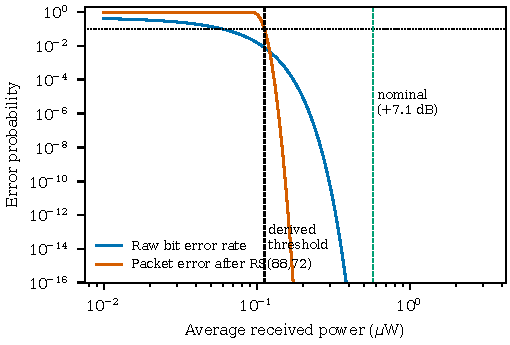
\includegraphics[width=\columnwidth]{figures/fig_v2_receiver.pdf}
\caption{Receiver model: raw bit-error rate and packet error after RS(88,72) versus average received power. The dashed lines mark the derived availability threshold and the nominal operating power.}
\label{fig:receiver}
\end{figure}

\subsection{Lock, Acquisition and Terminal Dynamics}
Each terminal tracks only while power stays above the threshold. A lock is lost after 0.5~s below it. Re-acquisition requires power at least 1.5 times the threshold for an acquisition dwell (3~s nominal, 15~s in a stress case), and a link carries packets only when both terminals are locked. The terminal is two cascaded 0.03~s lags with a 0.035~rad/s rate limit, tracking jitter $\sigma_\xi=10\urad$ RMS (35~$\mu$rad in a stress case), and encoder noise of $5\urad$. A local pilot dither and a Gaussian power fit estimate boresight bias; the fit-acceptance residual (0.20) was set on development seeds.

\begin{table}[!t]
\caption{Optical-layer parameters and their provenance}
\label{tab:optics}
\centering\footnotesize
\begin{tabular}{@{}p{0.40\columnwidth}p{0.52\columnwidth}@{}}
\toprule
Parameter & Value (source)\\
\midrule
Beam FWHM & $380\urad$ (NASA TBIRD, on-orbit measurement~\cite{schieler2023})\\
Body pointing jitter & $<10\urad$ RMS nominal~\cite{schieler2023icsos}; $35\urad$ stress (20--35~$\mu$rad uplink tracking~\cite{schieler2023})\\
Pull-in time & 3~s nominal (assumed); 15~s stress (TBIRD 10--30~s~\cite{schieler2023})\\
Tx power / losses & 5~mW; $-1$~dB Tx, $-5.2$~dB Rx (design, assumed)\\
Receiver, code & responsivity 0.9~A/W, 5~pA/$\sqrt{\text{Hz}}$, 100~Mbps OOK; RS(88,72) (design)\\
Lock hysteresis & 0.5~s loss hold, $1.5\times$ re-acquire (assumed)\\
Derived threshold & 0.112~$\mu$W at packet error 0.1\\
\bottomrule
\end{tabular}
\end{table}

\subsection{Validation Against Published NASA Data}
Table~\ref{tab:tbird} reproduces the downlink irradiance budget published for TBIRD at $30^\circ$ elevation~\cite{schieler2023} with the same budget function the crosslink simulator calls. The model total of $-52.97$~dB\,W/m$^2$ differs from the published $-52.9$ by 0.07~dB, and no line item differs by more than 0.15~dB.

\begin{table}[!t]
\caption{TBIRD downlink irradiance budget: published~\cite{schieler2023} versus the simulator's budget code}
\label{tab:tbird}
\centering\footnotesize
\begin{tabular}{@{}lrrr@{}}
\toprule
Item & Published & Model & Diff.\\
\midrule
Tx optical power, 0.9~W (dBW) & $-0.5$ & $-0.46$ & 0.04\\
Tx optics loss (dB) & $-0.3$ & $-0.30$ & 0.00\\
Tx gain, 380~$\mu$rad (dBi) & 79.0 & 78.85 & $-0.15$\\
Pointing loss, 50~$\mu$rad (dB) & $-0.2$ & $-0.21$ & $-0.01$\\
Range loss, 930~km (dB/m$^2$) & $-130.4$ & $-130.36$ & 0.04\\
Atmospheric loss (dB) & $-0.5$ & $-0.50$ & 0.00\\
\midrule
Irradiance (dB\,W/m$^2$) & $-52.9$ & $-52.97$ & $-0.07$\\
\bottomrule
\end{tabular}
\end{table}

\emph{What is real and what is modelled.} The budget, beam width, jitter range, pull-in range and the existence of a hard FEC threshold (about $-38$~dBm in the 200~Gbps mode) are published NASA/MIT-LL values. The 1~km crosslink geometry, the 100~Mbps receiver, the RS code, the lock thresholds and the transmitter power are modelled. Raw flight telemetry from NASA is not public, and we found no public ISRO inter-satellite-link data, so none is used. The validation therefore tests the link-budget arithmetic and calibrates the model; it is not a validation of the whole closed loop against flight data.



\section{Certificate}\label{sec:cert}
For spacecraft $i$ define the attitude and transported rate errors against the true desired state,
\begin{equation}
\chi_i=\|\Log(q_i^{\star*}\!\otimes q_i)\|,\quad
\epsilon_i=\|\omega_i-R(q_i)^TR(q_i^\star)\omega_i^\star\|.
\end{equation}
Let a packet from $j$ stamped $\tau$ carry $(q_j,\omega_j)$ and bounds $\chi_j\le H$, $\epsilon_j\le W$ at $\tau$. At $t=\tau+a$ spacecraft $i$ forms, with $\rho=o_j^*\otimes o_i$ and horizon $h\ge0$, the target
\begin{equation}
\begin{aligned}q_{t}(a)&=q_j\otimes\Exp(\omega_j\min(a,h))\otimes\rho,\\ \omega_{t}&=\begin{cases}R(\rho)^T\omega_j,&a<h\\ 0,&a\ge h.\end{cases}\end{aligned}
\end{equation}
For $a<h$ define
\begin{align}
E(a)&=e^{\bar\omega a}\big(H(1+\bar\omega a)+Wa+\bar\alpha a^2/2\big),\\
F(a)&=W+\bar\alpha a+\bar\omega\,(E(a)+H),
\end{align}
and for $a\ge h$: $E(a)=E(h)+\bar\omega(a-h)$, $F(a)=\bar\omega$. ($E$ is continuous at $h$; $F$ jumps to $\bar\omega$ because the target rate becomes zero.)

\begin{lemma}[Extrapolation certificate]\label{lem:ext}
Under Assumption~\ref{as:ref}, the target error satisfies $\|\Log(q_i^{\star*}(t)\otimes q_t(a))\|\le E(a)$ and the target rate error $\|\omega_t-R(q_t)^TR(q_i^\star)\omega_i^\star\|\le F(a)$.
\end{lemma}
\begin{proof}
Write $A(s)=q_j\otimes\Exp(\omega_js)\otimes\rho$, with constant body rate $a_1=R(\rho)^T\omega_j$, and $B(s)=q_i^\star(\tau+s)$ with body rate $a_2(s)=\omega_i^\star(\tau+s)$. Since $o_i=o_j\otimes\rho$, $a_2(0)=R(\rho)^T\omega_j^\star(\tau)$ and $B(s)=q_j^\star(\tau+s)\otimes\rho$. Let $\mathcal E(s)=B(s)^*\otimes A(s)$ and $\theta(s)=\|\Log\mathcal E(s)\|$. The relative body rate of $\mathcal E$ is $a_1-R(\mathcal E)^Ta_2$ and $\theta$ is the distance to the identity in a bi-invariant metric, so $\theta'\le\|R(\mathcal E)a_1-a_2(s)\|$. At $s=0$, $\mathcal E(0)=\rho^*\otimes(q_j^{\star*}\otimes q_j)\otimes\rho$ has $\theta(0)=\chi_j\le H$, and
\begin{equation}
\begin{aligned}\|R(\mathcal E(0))a_1-a_2(0)\|&=\|R(q_j)\omega_j-R(q_j^\star)\omega_j^\star\|\\&=\epsilon_j\le W,\end{aligned}
\end{equation}
because rotations preserve norms. Put $\delta=R(\mathcal E(0))a_1-a_2(0)$, $\|\delta\|\le W$. For $s>0$,
\begin{equation}
\begin{aligned}R(\mathcal E(s))a_1-a_2(s)&=\big[R(\mathcal E(s))R(\mathcal E(0))^T-I\big]a_2(0)\\&\quad+\big[a_2(0)-a_2(s)\big]\\&\quad+R(\mathcal E(s))R(\mathcal E(0))^T\delta.\end{aligned}
\end{equation}
The first term has norm at most $\bar\omega(\theta(s)+\theta(0))$, since $\|(I-R)v\|\le\angle(R)\|v\|$ and the angle of $\mathcal E(s)\mathcal E(0)^*$ is at most $\theta(s)+\theta(0)$. The second is at most $\bar\alpha s$, the third at most $W$. Hence $\theta'(s)\le W+\bar\alpha s+\bar\omega(\theta(s)+H)$, and Gr\"onwall's inequality gives
\begin{equation}
\theta(s)\le e^{\bar\omega s}\theta(0)+\!\int_0^s\!e^{\bar\omega(s-u)}(W+\bar\alpha u+\bar\omega H)\,du\le E(s),
\end{equation}
using $(e^x-1)/\bar\omega\le s e^{x}$ and $(e^x-1-x)/\bar\omega^2\le (s^2/2)e^{x}$ with $x=\bar\omega s$. The same inequality bounds the rate error by $F(s)$ for $s<h$. For $a\ge h$ the target is frozen and the desired attitude moves by at most $\bar\omega$ per second, so $\theta(a)\le\theta(h)+\bar\omega(a-h)$; the target rate is $0$ and the desired rate is at most $\bar\omega$.
\end{proof}

\begin{theorem}[Online certificate]\label{thm:cert}
Let the leader use $H_1=\|\Log(q_{t,1}^*\otimes q_1)\|$ and $W_1$ its transported rate error to the exact target $q_{t,1}=q_1^\star$. For a follower $i$ with any parent $p$ (possibly time-varying), whose newest delivered packet carries $(H_p,W_p)$ and has age $a$, let
\begin{align}
H_i&=E(a)+\|\Log(q_{t,i}^*\otimes q_i)\|,\\
W_i&=F(a)+\|\omega_i-R(q_i)^TR(q_{t,i})\omega_{t,i}\|,
\end{align}
and $H_i=W_i=\infty$ if no packet has arrived. Then $\chi_i(t)\le H_i(t)$ and $\epsilon_i(t)\le W_i(t)$ for all $t$, under arbitrary delays, losses, outages and parent switches. The common-frame pair error $\vartheta_{ij}=\|\Log((q_i\otimes o_i^*)^*\otimes(q_j\otimes o_j^*))\|$ satisfies $\vartheta_{ij}\le H_i+H_j$.
\end{theorem}
\begin{proof}
Induct on time. Delivery takes at least one sample, so every bound stored in a packet was computed from strictly earlier ones; the base cases are the leader, whose target is exact, and $H=\infty$. If the sender's bounds hold at its stamp, Lemma~\ref{lem:ext} bounds the target error and target rate error by $E(a)$ and $F(a)$, whichever packet is newest, however old, and whichever parent supplied it. By the triangle inequality for the geodesic distance, $\chi_i\le\angle(q_i^{\star*}q_{t,i})+\angle(q_{t,i}^*q_i)\le H_i$. For rates,
\begin{equation}
\begin{aligned}\omega_i-R(q_i)^TR(q_i^\star)\omega_i^\star&=\big[\omega_i-R(q_i)^TR(q_{t,i})\omega_{t,i}\big]\\&\quad+R(q_i)^T\big[R(q_{t,i})\omega_{t,i}-R(q_i^\star)\omega_i^\star\big],\end{aligned}
\end{equation}
whose norm is at most $W_i$. For the pair error, $q_i\otimes o_i^*$ differs from $q_r$ by $\chi_i$ in angle, so $\vartheta_{ij}\le\chi_i+\chi_j$.
\end{proof}

\begin{remark}
No acyclicity of the parent graph is needed: a cycle without a leader-anchored packet keeps $H=\infty$, and finite bounds always trace back to the leader. The theorem bounds the error of the \emph{target} and, through the measured local error, of the state. It does not bound the local error: stability of the delayed, saturated feedback loop is not proved. If the local loop were input-to-state stable from target error to local error with a gain $\gamma$ (an assumption we neither prove nor test), $\chi_i$ would be bounded by $(1+\gamma)$ times the supremum of $E$ plus a decaying term. We do not claim this.
\end{remark}

\section{Guaranteed-Accuracy Triggering}\label{sec:gat}
\subsection{Tolerance Rule}
Let $E_c(a)=E(a)-H$ be the \emph{communication-induced} part of the certified target error ($E$ is increasing in $a$). After sending a packet carrying $(H,W)$ at time $\tau$, the sender computes
\begin{equation}
a^\ast=\min\{a:\,E_c(a)\ge\varepsilon\},
\end{equation}
by bisection on the bound alone, and sends the next packet at
\begin{equation}
\tau+\min\{T_{\max},\ \max\{T_{\min},\ a^\ast-d_m\}\},
\end{equation}
with delay margin $d_m=0.25$~s (the delay in our model never exceeds 0.2~s except in the network case), $T_{\min}=0.1$~s and $T_{\max}=2$~s. The receiver uses the horizon $h=\min\{3,\max\{0,(\bar\omega-W)/\bar\alpha\}\}$~s, the age at which extrapolation stops being better in the worst case than holding. The rule needs no measurement of the follower's state and no model of its controller.

\begin{proposition}[Tolerance guarantee]\label{prop:gat}
Suppose that on a link consecutive packets are delivered with delay at most $d_m$ and no packet in between is lost, and that $E_c(T_{\min}+d_m)\le\varepsilon$ (the tolerance is feasible). Then from the first delivery onward the receiver's certified target error satisfies $E_c(a)\le\varepsilon$ at every instant.
\end{proposition}
\begin{proof}
After a delivery of the packet stamped $\tau$ the receiver's age is the elapsed time since $\tau$. The next packet is sent no later than $\tau+\max\{T_{\min},a^\ast-d_m\}$ (or at $T_{\max}<a^\ast-d_m$) and arrives at most $d_m$ later, so before the age exceeds $\max\{T_{\min}+d_m,a^\ast\}$, and for $a\le a^\ast$ monotonicity gives $E_c(a)\le\varepsilon$; the case $T_{\min}+d_m>a^\ast$ is excluded by feasibility. Both ends compute $E_c$ from the same $(H,W)$, so the sender's prediction equals the receiver's bound.
\end{proof}
The guarantee is conditional: a lost packet, an outage or a delay above $d_m$ voids it, and the certificate then reports the actual bound. A child that switches parent also leaves the new parent unaware for a short time (Section~\ref{sec:results} measures this).

\subsection{Certified Parent Re-selection and Variants}
Each follower evaluates $E$ for the newest packet from every other spacecraft and uses the candidate with the smallest bound. It switches only when the best bound is below $0.8$ of the current one and the last switch is at least 2~s old, or when the current parent has no data. A parent learns that it is a parent from the child's report (every 2~s on the parent link; 6~s heartbeats on the others), and a terminal that is not locked retries every 1.6~s. \textbf{GAT} uses the tolerance rule on parent links with these reports; \textbf{GAT-fixed} keeps a static leader-fed star and no re-selection. \textbf{CLAC}, the authors' certified event-rule variant from earlier development, uses the same certificate and re-selection but sends on the innovation threshold of the authors' previous event rule ($150\urad$ attitude, $100\urad$/s rate) with 1~s reports and 3~s heartbeats; it has no tolerance guarantee.

\section{Baselines, Conditions and Protocol}\label{sec:protocol}
\subsection{Compared Methods}
All methods share the simulator, local controller, optical layer, seeds, disturbances and channel draws. They are adaptations, not the authors' original code.
\begin{itemize}
\item \textbf{Ideal}: periodic exchange with perfect delivery on the chain (reference only).
\item \textbf{Periodic}: 0.2~s exchange over the optical links with pilot recovery.
\item \textbf{EO chain, EO star}: the authors' previous event rule with prediction on the chain SC1$\to$SC2$\to$SC3$\to$SC4 and on a static star in which the leader feeds every follower. The star is included because a static tree better than the chain would otherwise inflate the benefit of re-selection.
\item \textbf{ETC}: static event trigger with zero-order hold~\cite{tabuada2007}. \textbf{DET}: dynamic event trigger with internal variable~\cite{girard2015} and the same predicting receiver. \textbf{ST}: self-triggered next time from a model-based deviation bound~\cite{mazo2010,heemels2012}.
\item \textbf{CLAC}, \textbf{GAT-fixed}, \textbf{GAT}.
\end{itemize}
Each baseline has one free parameter, set on development seeds 11/23/47 to the most accurate value whose mean payload does not exceed 1.05 times the payload of CLAC (76.7~kB), so the budget is a cap and not an equality. For GAT, the tolerance was set to $\varepsilon=1$~mrad, the largest grid value at which traffic still depends on $\varepsilon$ (above 2~mrad traffic saturates at the 2~s cap), and the report and heartbeat periods (2~s, 6~s) were chosen because 1~s and 3~s added 13~kB for under 1\% accuracy. Fig.~\ref{fig:dial} shows the development sweeps.

\begin{figure}[!t]
\centering
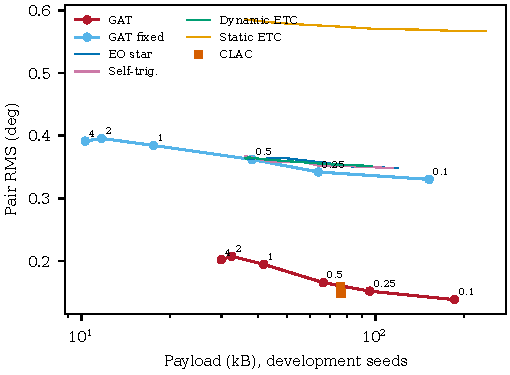
\includegraphics[width=\columnwidth]{figures/fig_v3_dial.pdf}
\caption{Development seeds: pair RMS against payload for the tolerance sweep of GAT (numbers: $\varepsilon$ in mrad) and the baselines' parameter sweeps. Baseline accuracy changes little with payload.}
\label{fig:dial}
\end{figure}

\subsection{Conditions}
Seventeen conditions are used; the fault window is 35~s (25--60~s) except for combined (28--52~s), severe attenuation (22--55~s) and beam mismatch (20--58~s). The 14 conditions of the earlier study are: healthy; pointing bias on one link; pointing bias with three different vectors on the three chain links; bias on all six links; an \emph{isolated} actuator fault (SC2 effectiveness $0.30/0.45/0.35$, optics untouched); severe attenuation of link 1--2 (gain 0.08); combined pointing, attenuation and actuator faults; a beam 10\% narrower than modelled; an alternate tree with 0.2~s delay and 10\% extra loss; 35~$\mu$rad jitter; 15~s pull-in; pointing bias on a random link; outage of a random link; outage of two random links. Three conditions are new and were never used in tuning or any earlier run (marked $*$): a pointing bias that ramps to $1.4\times$ on a random link, intermittent outages (3~s every 8~s) of a random link, and a random-link outage combined with a degraded actuator on SC3. Only five condition types (one-link pointing, combined, random-link pointing, random-link outage, actuator only) were used for tuning, on seeds 11/23/47. In the random-link conditions the faulty links are drawn from the seed (the held-out seeds balance the six links) and are identical for every method.

\subsection{Seeds, Lock and Statistics}
The 20 held-out seeds are 401--420, never used before (the earlier study used 201--220). Each seed fixes initial attitudes and rates, the reference phase, disturbances and fault location. Sources, tuning outputs and protocol were hashed (SHA-256) before the run. The in-metric check of the rate certificate then flagged four of 1{,}020 certified runs (network condition, GAT and GAT-fixed, seeds 409 and 417): at a follower age of exactly 3.00~s, the horizon cap, the controller already holds the target while the rate bound still used the extrapolating branch. This was a boundary bug in both the lemma statement and the code; the attitude bound was not affected. We fixed it (Section~\ref{sec:cert} now defines $F(a)=\bar\omega$ for $a\ge h$), locked again, and re-ran all 3{,}400 runs on the same seeds. The corrected run has the same pair RMS and attempts in every run as the first one, and zero violations. Both locks and the first results are kept in the repository. The earlier 560 trajectories (280 CLAC, 280 CLAC-fixed) re-run with the fix give zero violations and change one run by 0.1\%. The primary outcome is the fault-window pair RMS (degrees). Intervals are 95\% percentile bootstrap intervals over seeds (10{,}000 resamples, paired across methods), exploratory and unadjusted for multiplicity. An independent recomputation reproduced all 900 means to $4\times10^{-16}$ relative and all interval ends within 0.04 interval widths.

\section{Results}\label{sec:results}
\subsection{Accuracy and Traffic}
Table~\ref{tab:pair} and Fig.~\ref{fig:pair} give pair RMS; Table~\ref{tab:cost} and Fig.~\ref{fig:tradeoff} give payload; Table~\ref{tab:contrast} gives GAT's paired change against the main baselines.

\begin{table*}[!t]
\caption{Fault-window pair RMS (deg), mean over 20 held-out seeds (seeds 401--420). Bold: best among the event-based methods (not Ideal/Periodic). Per.: periodic; ETC/DET/ST: static, dynamic, self-triggered; GAT-F: GAT without re-selection. $*$: condition never used before. ``Ideal'' (0.334$^\circ$ mean) uses the chain and is not a lower bound over topologies.}
\label{tab:pair}
\centering\scriptsize
\begin{tabular}{@{}lrrrrrrrrr@{\,}l@{}}
\toprule
Condition & Per. & EO ch. & EO st. & ETC & DET & ST & CLAC & GAT-F & GAT & \multicolumn{1}{c}{GAT 95\% CI}\\
\midrule
Healthy & 0.356 & 0.376 & 0.117 & 0.462 & 0.115 & \textbf{0.115} & 0.117 & 0.152 & 0.153 & [0.149, 0.158]\\
Pointing, 1 link & 0.387 & 0.411 & 0.185 & 0.475 & 0.182 & 0.170 & \textbf{0.138} & 0.205 & 0.187 & [0.174, 0.199]\\
Pointing, 3 links & 0.450 & 0.478 & 0.185 & 0.475 & 0.182 & 0.170 & \textbf{0.144} & 0.205 & 0.193 & [0.182, 0.205]\\
Pointing, 6 links & 0.469 & 0.501 & 0.212 & 0.496 & 0.207 & 0.196 & \textbf{0.170} & 0.246 & 0.241 & [0.217, 0.265]\\
Actuator only & 0.366 & 0.385 & 0.120 & 0.462 & 0.118 & \textbf{0.118} & 0.120 & 0.156 & 0.156 & [0.152, 0.161]\\
Severe attenuation & 1.118 & 1.123 & 1.147 & 1.069 & 1.146 & 1.150 & \textbf{0.196} & 1.143 & 0.263 & [0.250, 0.277]\\
Combined & 0.396 & 0.427 & 0.231 & 0.504 & 0.227 & 0.233 & \textbf{0.153} & 0.236 & 0.221 & [0.205, 0.236]\\
Beam mismatch & 0.481 & 0.503 & 0.257 & 0.473 & 0.255 & 0.248 & \textbf{0.149} & 0.303 & 0.203 & [0.185, 0.226]\\
Network transfer & 0.492 & 0.544 & 0.206 & 0.487 & 0.196 & 0.185 & \textbf{0.155} & 0.240 & 0.219 & [0.208, 0.228]\\
35 $\mu$rad jitter & 1.179 & 1.200 & 1.099 & 1.064 & 1.098 & 1.092 & \textbf{0.353} & 1.086 & 0.433 & [0.348, 0.533]\\
15 s pull-in & 1.016 & 1.041 & 0.698 & 0.707 & 0.693 & 0.675 & \textbf{0.356} & 0.683 & 0.435 & [0.352, 0.522]\\
Pointing, random link & 0.403 & 0.424 & 0.151 & 0.468 & 0.148 & 0.142 & \textbf{0.131} & 0.182 & 0.171 & [0.160, 0.182]\\
Outage, random link & 0.876 & 0.892 & 0.661 & 0.791 & 0.657 & 0.653 & \textbf{0.162} & 0.670 & 0.205 & [0.183, 0.226]\\
Outage, two links & 1.133 & 1.144 & 1.081 & 1.075 & 1.078 & 1.071 & \textbf{0.206} & 1.065 & 0.270 & [0.239, 0.305]\\
Pointing ramp* & 0.363 & 0.382 & 0.117 & 0.462 & 0.115 & \textbf{0.115} & 0.117 & 0.152 & 0.153 & [0.149, 0.158]\\
Intermittent outage* & 0.482 & 0.507 & 0.282 & 0.500 & 0.271 & 0.268 & \textbf{0.159} & 0.288 & 0.211 & [0.186, 0.237]\\
Outage + actuator* & 0.883 & 0.900 & 0.664 & 0.792 & 0.660 & 0.656 & \textbf{0.167} & 0.673 & 0.210 & [0.188, 0.233]\\
\midrule
Mean of 17 & 0.638 & 0.661 & 0.436 & 0.633 & 0.432 & 0.427 & \textbf{0.176} & 0.452 & 0.231 & [0.220, 0.242]\\
\bottomrule
\end{tabular}

\end{table*}

\begin{figure*}[!t]
\centering
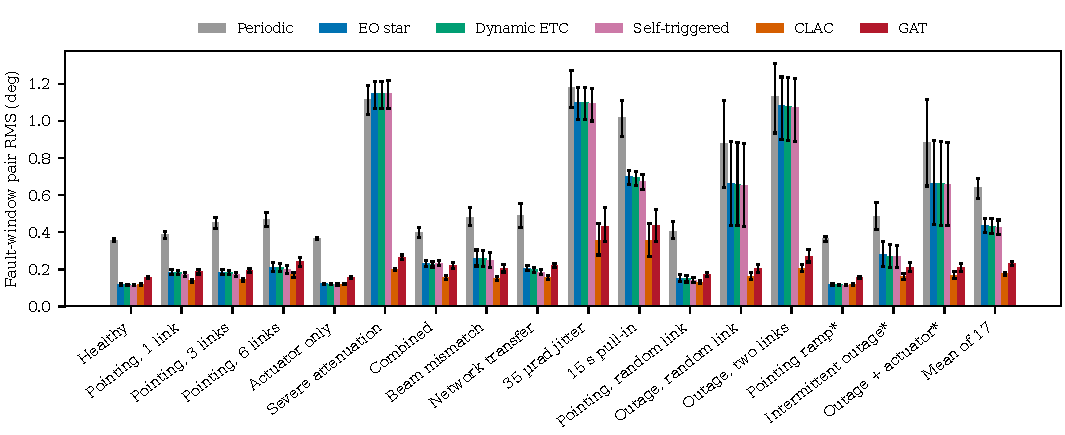
\includegraphics[width=\textwidth]{figures/fig_v3_pair.pdf}
\caption{Pair RMS with 95\% bootstrap intervals (20 held-out seeds) for six methods in 17 conditions and their mean.}
\label{fig:pair}
\end{figure*}

\begin{table}[!t]
\caption{Mean over the 17 conditions: payload, attempted packets, pair RMS (95\% CI).}
\label{tab:cost}
\centering\footnotesize
\begin{tabular}{@{}lrrr@{}}
\toprule
Method & Payload (kB) & Attempts & Pair RMS (deg)\\
\midrule
Ideal communication & 144.0 & 2250 & 0.334 [0.327, 0.343]\\
Periodic & 144.0 & 2250 & 0.638 [0.582, 0.691]\\
EO, chain & 82.1 & 1282 & 0.661 [0.604, 0.715]\\
EO, star & 68.5 & 1070 & 0.436 [0.397, 0.475]\\
Static ETC (ZOH) & 74.8 & 1169 & 0.633 [0.612, 0.655]\\
Dynamic ETC & 71.6 & 1118 & 0.432 [0.394, 0.471]\\
Self-triggered & 72.2 & 1128 & 0.427 [0.388, 0.466]\\
CLAC & 78.6 & 893 & 0.176 [0.168, 0.185]\\
GAT, no re-selection & 18.0 & 204 & 0.452 [0.413, 0.492]\\
GAT & 44.4 & 505 & 0.231 [0.220, 0.242]\\
\bottomrule
\end{tabular}

\end{table}

\begin{figure}[!t]
\centering
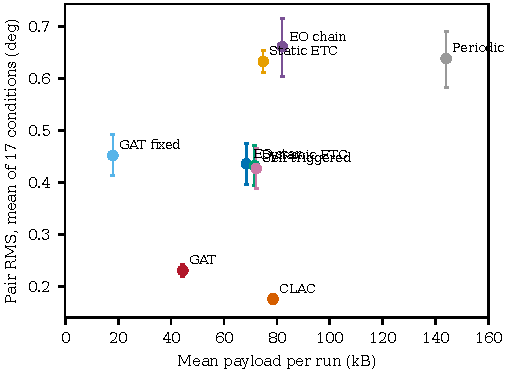
\includegraphics[width=\columnwidth]{figures/fig_v3_tradeoff.pdf}
\caption{Accuracy against payload (mean of 17 conditions, 95\% interval on pair RMS).}
\label{fig:tradeoff}
\end{figure}

\begin{table*}[!t]
\caption{GAT minus baseline: paired change in pair RMS (\%), mean [95\% CI]. Negative favours GAT.}
\label{tab:contrast}
\centering\scriptsize
\begin{tabular}{@{}lrrrr@{}}
\toprule
Condition & vs EO star & vs DET & vs ST & vs CLAC\\
\midrule
Healthy & 30.7 [29.7, 31.9] & 32.8 [31.8, 34.1] & 33.4 [32.4, 34.7] & 30.8 [30.0, 32.0]\\
Pointing, 1 link & 2.5 [-4.7, 9.3] & 4.1 [-2.8, 10.9] & 10.6 [4.3, 16.6] & 35.3 [30.2, 41.3]\\
Pointing, 3 links & 5.9 [-0.6, 11.9] & 7.7 [1.3, 13.9] & 14.4 [8.6, 19.7] & 34.8 [30.4, 39.5]\\
Pointing, 6 links & 15.5 [8.5, 22.4] & 17.6 [11.2, 24.0] & 24.2 [17.8, 30.8] & 42.0 [34.2, 49.8]\\
Actuator only & 29.9 [28.9, 31.1] & 32.0 [31.0, 33.3] & 32.6 [31.6, 33.9] & 30.0 [29.1, 31.2]\\
Severe attenuation & -76.7 [-78.2, -75.0] & -76.7 [-78.1, -75.1] & -76.8 [-78.2, -75.2] & 34.1 [28.4, 40.4]\\
Combined & -3.0 [-10.2, 3.2] & -1.3 [-9.0, 5.8] & -4.0 [-11.4, 2.4] & 45.4 [37.3, 53.6]\\
Beam mismatch & -13.8 [-24.9, -3.1] & -13.0 [-24.1, -2.1] & -10.6 [-22.0, 0.5] & 35.9 [30.1, 42.4]\\
Network transfer & 9.1 [-0.2, 19.4] & 14.0 [6.2, 22.9] & 20.1 [13.1, 28.1] & 42.6 [35.7, 49.7]\\
35 $\mu$rad jitter & -59.6 [-67.7, -50.3] & -59.7 [-67.7, -50.6] & -59.3 [-67.5, -50.0] & 36.9 [12.2, 64.3]\\
15 s pull-in & -37.7 [-49.0, -26.2] & -37.1 [-48.6, -25.4] & -35.4 [-47.1, -23.4] & 34.3 [21.1, 49.2]\\
Pointing, random link & 17.6 [8.9, 25.1] & 19.6 [10.7, 27.2] & 23.3 [16.4, 29.2] & 30.5 [26.7, 34.3]\\
Outage, random link & -28.7 [-51.1, -6.5] & -27.6 [-50.6, -5.0] & -27.2 [-50.3, -4.5] & 27.1 [24.1, 30.3]\\
Outage, two links & -64.9 [-76.6, -49.0] & -64.6 [-76.5, -48.5] & -64.3 [-76.4, -48.1] & 31.5 [23.5, 44.6]\\
Pointing ramp* & 30.7 [29.7, 31.9] & 32.8 [31.8, 34.1] & 33.4 [32.4, 34.7] & 30.8 [30.0, 32.0]\\
Intermittent outage* & -6.9 [-22.5, 8.3] & -4.7 [-20.0, 10.2] & -3.7 [-19.2, 11.3] & 33.0 [26.7, 42.2]\\
Outage + actuator* & -28.7 [-50.9, -6.7] & -27.7 [-50.3, -5.3] & -27.3 [-50.0, -4.8] & 26.5 [23.4, 29.8]\\
\midrule
Mean of 17 & -45.1 [-49.9, -39.8] & -44.8 [-49.4, -39.6] & -43.9 [-48.7, -38.5] & 31.4 [28.0, 34.8]\\
\bottomrule
\end{tabular}

\end{table*}

\emph{Tolerance triggering alone (GAT-fixed).} On the same static star, GAT-fixed sends 18.0~kB against 68.5~kB for the tuned event trigger: 73.6\% less (CI $[71.7,75.3]\%$ less), and 75.1\% less than the self-triggered rule. The mean pair RMS is only 4.0\% higher (CI $[1.6,6.3]\%$). The mean hides a split: when nothing fails, GAT-fixed is 30.0\% worse than EO star (0.152$^\circ$ against 0.117$^\circ$) at 73.1\% less payload, and in outage conditions every star-based method fails alike, so the means are close.

\emph{With certified re-selection (GAT).} Over the 17 conditions GAT lowers pair RMS by 45.1\% against EO star (CI $[39.8,49.9]\%$), 44.8\% against DET and 43.9\% against ST (CI $[38.5,48.7]\%$), while sending 34.9\%, 37.9\% and 38.5\% less payload. The gain comes from link faults: under severe attenuation of link 1--2 GAT reaches $0.263^\circ$ against $1.147^\circ$ for EO star (76.7\% lower); with a random-link outage 28.7\% lower (CI $[6.5,51.1]\%$), two-link outage 64.9\%, 35~$\mu$rad jitter 59.6\% and 15~s pull-in 37.7\% lower.

\emph{Where GAT loses.} With no link fault GAT is 30.7\% worse than EO star (CI $[29.7,31.9]\%$) and 33\% worse than DET and ST, because the tolerance at $\varepsilon=1$~mrad lets the follower run on extrapolated targets. Against CLAC, GAT is 31.4\% worse (CI $[28.0,34.8]\%$) over the 17 conditions while sending 43.4\% less: CLAC is the more accurate and GAT the leaner method. The pointing bias that ramps slowly is absorbed by the terminal's pilot recovery in every method (the row equals the healthy row).

\emph{Unseen conditions.} On the three conditions never used before, CLAC is 24.7\% lower than EO star (CI $[15.4,34.1]\%$), whereas GAT is only 1.6\% lower with an interval that includes zero ($[-14.2,+10.5]\%$ averaged over the three; ramp equals healthy, intermittent outage $-6.9\%$, CI $[-22.2,+8.1]\%$, and outage plus actuator $-28.7\%$, CI $[-50.9,-6.9]\%$). The advantage of GAT over the event trigger therefore needs a hard link fault.

\emph{Isolated actuator fault.} The actuator-only condition raises pair RMS by 0.010$^\circ$ for ideal communication relative to healthy and by 0.003$^\circ$ for GAT: the feedback and disturbance estimator absorb it. A harsher actuator fault was not tested.

\begin{figure}[!t]
\centering
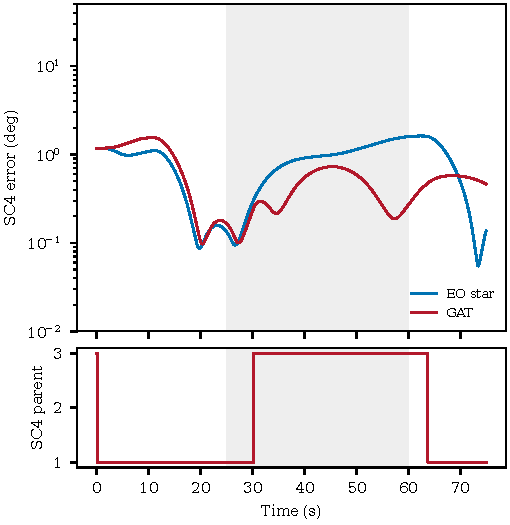
\includegraphics[width=\columnwidth]{figures/fig_v3_trace.pdf}
\caption{SC4 error and GAT parent choice when the SC1--SC4 link is out (shaded; seed 403). The static star loses its leader link; GAT moves SC4 to another spacecraft and returns after the link re-locks.}
\label{fig:trace}
\end{figure}

\subsection{Guarantee and Certificate}
In healthy runs on locked links the tolerance held in 99.5\% of samples for GAT-fixed and 99.2\% for GAT in the fault-free window ($t\ge10$~s before the fault); over all 17 conditions, restricted to locked parent links, in 98.3\% and 96.3\%. The shortfall comes from the transient after a parent switch (the new parent has not yet learned that it is a parent) and from losses. Neither the attitude nor the rate certificate was violated in 1{,}020 held-out trajectories (340 each of CLAC, GAT-fixed and GAT); the median over GAT runs of the per-run median ratio of actual to certified error is 0.92, because the bound adds the exact local error to the extrapolation bound. GAT changed parent 4.2 times per run on average.

\section{Discussion}
Tolerance triggering is easy to state: one number with a unit sets the traffic, and the bound reports the guarantee's status. Its cost is accuracy when nothing fails, because a tolerance that is safe in the worst case is loose in the typical case; the event rule uses the actual deviation and is more accurate per byte near 77~kB (CLAC). The re-selection, driven by the same bound, is what makes both methods robust to link faults, and it is the same idea under both. The advantage over event triggering is clear for hard link faults and absent for slow pointing drift.

\section{Limitations and Threats to Validity}\label{sec:limits}
\begin{itemize}
\item \textbf{Closed-loop stability is not proved.} The certificate bounds the target error and, through the measured local error, the state error. The ISS-type corollary in the remark is an assumption.
\item \textbf{Simulation only.} There is no hardware-in-the-loop, flight or second high-fidelity simulator. Only published TBIRD values calibrate the model, a 930~km downlink, not a 1~km crosslink; raw NASA telemetry is not public and no ISRO crosslink data were found.
\item \textbf{The command class is assumed known}; a wrong $\bar\omega$ or $\bar\alpha$ breaks the certificate. The constants were checked numerically.
\item \textbf{Baselines are adaptations}, each tuned with one parameter on five condition types. Other tuning or stronger triggers could narrow the gaps; faulty-link conditions favour any method that can change its tree. The tolerance guarantee is conditional on delivery.
\item \textbf{Same team, same simulator} for tuning and evaluation. The held-out seeds are fresh and three conditions are unseen, but the unseen conditions are variants of known fault types.
\item \textbf{Novelty} is stated relative to the literature we reviewed; absence of prior work cannot be proved.
\item \textbf{Defect disclosure.} A boundary bug in the rate bound was found by our own check after the first lock and fixed (Section~\ref{sec:protocol}).
\end{itemize}

\section{Conclusion}
A bound that travels with each packet turns two decisions, when to send and whom to listen to, into computations the nodes make from the command-generator limits alone. The tolerance rule cuts traffic by about three quarters at a small average accuracy cost, and with re-selection it cuts the pair error of the budget-matched baselines under link faults, but it does not improve fault-free accuracy and it does not beat the event trigger on the unseen drift and intermittent conditions. What remains open is a closed-loop stability proof for the saturated delayed controller, hardware or independent high-fidelity validation, and calibration with crosslink data when such data become public.

\section*{Data and Software Availability}
Code, configurations, tuning sweeps, both lock files, result CSVs, analysis scripts and tests are in the project repository (\url{https://github.com/kaushalrog/Satellite-Optical-Fault-Recovery}, branch \texttt{gat-method}). MATLAB R2026a runs \texttt{run\_tests\_all} and \texttt{run\_v3\_evaluation}; Python scripts regenerate all tables and figures. The NASA values come from the cited public reports.

\section*{Acknowledgment}
The authors thank the Amrita School of Artificial Intelligence for support.

\begin{thebibliography}{99}
\bibitem{click} NASA, ``CubeSat Laser Infrared CrosslinK (CLICK),'' NASA Small Spacecraft mission description, accessed Oct. 22, 2026. [Online]. Available: \url{https://www.nasa.gov/smallspacecraft/what-is-click/}
\bibitem{liu2018} G.-P. Liu and S. Zhang, ``A survey on formation control of small satellites,'' \emph{Proc. IEEE}, vol. 106, no. 3, pp. 440--457, 2018.
\bibitem{cai2014} H. Cai and J. Huang, ``The leader-following attitude control of multiple rigid spacecraft systems,'' \emph{Automatica}, vol. 50, no. 4, pp. 1109--1115, 2014.
\bibitem{wang2021} S. Wang, Z. Shu, and T. Chen, ``Event-triggered attitude synchronization of multiple rigid-body systems,'' \emph{Syst. Control Lett.}, vol. 149, p. 104879, 2021.
\bibitem{xie2023} X. Xie, T. Sheng, and X. Chen, ``Self-triggered formation control for multi-spacecraft attitude coordination with communication delays,'' \emph{J. Franklin Inst.}, vol. 360, no. 18, pp. 14696--14711, 2023.
\bibitem{xie2024asr} X. Xie, T. Sheng, and X. Chen, ``Self-triggered formation attitude control for multiple spacecraft with disturbances,'' \emph{Adv. Space Res.}, vol. 74, no. 3, pp. 1288--1299, 2024.
\bibitem{jia2023} Q. Jia, J. Gao, C. Zhang, C. K. Ahn, and D. Yu, ``Dynamic event-triggered attitude synchronization of multi-spacecraft formation via a learning neural network control approach,'' \emph{Aerosp. Sci. Technol.}, vol. 142, p. 108653, 2023.
\bibitem{xie2024taes} X. Xie, T. Sheng, and X. Chen, ``Dynamic event-triggered and self-triggered fault-tolerant attitude control for multiple spacecraft systems with uncertainties and input saturation,'' \emph{IEEE Trans. Aerosp. Electron. Syst.}, vol. 60, no. 3, pp. 2922--2933, Jun. 2024, doi: 10.1109/TAES.2024.3355381.
\bibitem{ren2007} W. Ren, ``Distributed attitude alignment in spacecraft formation flying,'' \emph{Int. J. Adapt. Control Signal Process.}, vol. 21, no. 2-3, pp. 95--113, 2007, doi: 10.1002/acs.916.
\bibitem{sarlette2009} A. Sarlette, R. Sepulchre, and N. E. Leonard, ``Autonomous rigid body attitude synchronization,'' \emph{Automatica}, vol. 45, no. 2, pp. 572--577, 2009, doi: 10.1016/j.automatica.2008.09.020.
\bibitem{abdessameud2009} A. Abdessameud and A. Tayebi, ``Attitude synchronization of a group of spacecraft without velocity measurements,'' \emph{IEEE Trans. Autom. Control}, vol. 54, no. 11, pp. 2642--2648, 2009, doi: 10.1109/TAC.2009.2031567.
\bibitem{mayhew2011} C. G. Mayhew, R. G. Sanfelice, and A. R. Teel, ``Quaternion-based hybrid control for robust global attitude tracking,'' \emph{IEEE Trans. Autom. Control}, vol. 56, no. 11, pp. 2555--2566, 2011, doi: 10.1109/TAC.2011.2108490.
\bibitem{dimarogonas2009} D. V. Dimarogonas, P. Tsiotras, and K. J. Kyriakopoulos, ``Leader--follower cooperative attitude control of multiple rigid bodies,'' \emph{Syst. Control Lett.}, vol. 58, no. 6, pp. 429--435, 2009.
\bibitem{tabuada2007} P. Tabuada, ``Event-triggered real-time scheduling of stabilizing control tasks,'' \emph{IEEE Trans. Autom. Control}, vol. 52, no. 9, pp. 1680--1685, 2007, doi: 10.1109/TAC.2007.904277.
\bibitem{girard2015} A. Girard, ``Dynamic triggering mechanisms for event-triggered control,'' \emph{IEEE Trans. Autom. Control}, vol. 60, no. 7, pp. 1992--1997, 2015, doi: 10.1109/TAC.2014.2366855.
\bibitem{heemels2012} W. Heemels, K. Johansson, and P. Tabuada, ``An introduction to event-triggered and self-triggered control,'' in \emph{Proc. 51st IEEE Conf. Decision Control (CDC)}, 2012, pp. 3270--3285.
\bibitem{nowzari2019} C. Nowzari, E. Garcia, and J. Cort\'es, ``Event-triggered communication and control of networked systems for multi-agent consensus,'' \emph{Automatica}, vol. 105, pp. 1--27, 2019, doi: 10.1016/j.automatica.2019.03.009.
\bibitem{heemels2013} W. P. M. H. Heemels, M. C. F. Donkers, and A. R. Teel, ``Periodic event-triggered control for linear systems,'' \emph{IEEE Trans. Autom. Control}, vol. 58, no. 4, pp. 847--861, 2013, doi: 10.1109/TAC.2012.2220443.
\bibitem{mazo2010} M. Mazo, Jr., A. Anta, and P. Tabuada, ``An ISS self-triggered implementation of linear controllers,'' \emph{Automatica}, vol. 46, no. 8, pp. 1310--1314, 2010, doi: 10.1016/j.automatica.2010.05.009.
\bibitem{donkers2012} M. C. F. Donkers and W. P. M. H. Heemels, ``Output-based event-triggered control with guaranteed $\mathcal{L}_\infty$-gain and improved and decentralized event-triggering,'' \emph{IEEE Trans. Autom. Control}, vol. 57, no. 6, pp. 1362--1376, 2012, doi: 10.1109/TAC.2011.2174696.
\bibitem{olfati2007} R. Olfati-Saber, J. A. Fax, and R. M. Murray, ``Consensus and cooperation in networked multi-agent systems,'' \emph{Proc. IEEE}, vol. 95, no. 1, pp. 215--233, 2007, doi: 10.1109/JPROC.2006.887293.
\bibitem{hespanha2007} J. P. Hespanha, P. Naghshtabrizi, and Y. Xu, ``A survey of recent results in networked control systems,'' \emph{Proc. IEEE}, vol. 95, no. 1, pp. 138--162, 2007.
\bibitem{zhang2001} W. Zhang, M. S. Branicky, and S. M. Phillips, ``Stability of networked control systems,'' \emph{IEEE Control Syst. Mag.}, vol. 21, no. 1, pp. 84--99, 2001, doi: 10.1109/37.898794.
\bibitem{sinopoli2004} B. Sinopoli, L. Schenato, M. Franceschetti, K. Poolla, M. I. Jordan, and S. S. Sastry, ``Kalman filtering with intermittent observations,'' \emph{IEEE Trans. Autom. Control}, vol. 49, no. 9, pp. 1453--1464, 2004, doi: 10.1109/TAC.2004.834121.
\bibitem{kaymak2018} Y. Kaymak, R. Rojas-Cessa, J. Feng, N. Ansari, M. Zhou, and T. Zhang, ``A survey on acquisition, tracking, and pointing mechanisms for mobile free-space optical communications,'' \emph{IEEE Commun. Surveys Tuts.}, vol. 20, no. 2, pp. 1104--1123, 2018.
\bibitem{kaushal2017} H. Kaushal and G. Kaddoum, ``Optical communication in space: Challenges and mitigation techniques,'' \emph{IEEE Commun. Surveys Tuts.}, vol. 19, no. 1, pp. 57--96, 2017.
\bibitem{toyoshima2005} M. Toyoshima, ``Trends in satellite communications and the role of optical free-space communications [Invited],'' \emph{J. Opt. Netw.}, vol. 4, no. 6, pp. 300--311, 2005, doi: 10.1364/JON.4.000300.
\bibitem{farid2007} A. A. Farid and S. Hranilovic, ``Outage capacity optimization for free-space optical links with pointing errors,'' \emph{J. Lightw. Technol.}, vol. 25, no. 7, pp. 1702--1710, 2007, doi: 10.1109/JLT.2007.899174.
\bibitem{khalighi2014} M. A. Khalighi and M. Uysal, ``Survey on free space optical communication: A communication theory perspective,'' \emph{IEEE Commun. Surveys Tuts.}, vol. 16, no. 4, pp. 2231--2258, 2014, doi: 10.1109/COMST.2014.2329501.
\bibitem{schieler2023} C. M. Schieler \emph{et al.}, ``On-orbit demonstration of 200-Gbps laser communication downlink from the TBIRD CubeSat,'' in \emph{Proc. SPIE}, 2023, NASA Tech. Rep. NTRS 20230000434. [Online]. Available: \url{https://ntrs.nasa.gov/citations/20230000434}
\bibitem{schieler2023icsos} C. M. Schieler \emph{et al.}, ``Recent on-orbit results and ARQ performance analysis for the TBIRD 200-Gbps mission,'' in \emph{Proc. Int. Conf. Space Opt. Syst. Appl. (ICSOS)}, 2023, NASA Tech. Rep. NTRS 20230014010. [Online]. Available: \url{https://ntrs.nasa.gov/citations/20230014010}
\bibitem{reed1960} I. S. Reed and G. Solomon, ``Polynomial codes over certain finite fields,'' \emph{J. Soc. Ind. Appl. Math.}, vol. 8, no. 2, pp. 300--304, 1960.
\bibitem{zhang2008} Y. Zhang and J. Jiang, ``Bibliographical review on reconfigurable fault-tolerant control systems,'' \emph{Annu. Rev. Control}, vol. 32, no. 2, pp. 229--252, 2008, doi: 10.1016/j.arcontrol.2008.03.008.
\bibitem{heirung2019} T. A. N. Heirung and A. Mesbah, ``Input design for active fault diagnosis,'' \emph{Annu. Rev. Control}, vol. 47, pp. 35--50, 2019, doi: 10.1016/j.arcontrol.2019.03.002.
\bibitem{scott2014} J. K. Scott, R. Findeisen, R. D. Braatz, and D. M. Raimondo, ``Input design for guaranteed fault diagnosis using zonotopes,'' \emph{Automatica}, vol. 50, no. 6, pp. 1580--1589, 2014, doi: 10.1016/j.automatica.2014.03.016.
\bibitem{raimondo2016} D. M. Raimondo, G. R. Marseglia, R. D. Braatz, and J. K. Scott, ``Closed-loop input design for guaranteed fault diagnosis using set-valued observers,'' \emph{Automatica}, vol. 74, pp. 107--117, 2016, doi: 10.1016/j.automatica.2016.07.033.
\end{thebibliography}
\end{document}

